% Provenance (never printed): see sources/outline_sources.md (Year 3:
% moments of inertia and gravity fields; impact cratering and crater dating;
% volcanism and tectonics on Mars, Venus, Io and the icy moons).
% Brief: sources/book5/BRIEFS.md, ch. 26. Curves from figdata/bachelor-3/
% two_layer_planet.py (two-layer interiors of the Earth, Mars, the Moon and
% Mercury from mean density and moment of inertia) and crater_sfd.py
% (the Ivanov production function and the Hartmann-Neukum chronology of
% Mars from the Craterstats configuration, the lunar chronology of Neukum,
% Hartmann's equilibrium density, and two invented Martian plains whose
% counts are drawn once from a Poisson law). Exercise and problem values in
% the Book 5 scratch calculator calc/ch26.py. Plains A and B are invented.
\chapter{行星内部与表面}\label{ch:b3:planetary-interiors-surfaces}

透过双筒望远镜看月球，可以发现它有两种地貌。明亮的
高地布满撞击坑，坑叠着坑：它们曾被
大型撞击坑饱和，这场强烈轰击约在 38 亿年前结束。
暗色的月海是充满熔岩的平原，形成于 42 亿至
12 亿年前，撞击坑却少得多。阿波罗号与月球号
任务从两类地貌带回岩石，其放射性年龄把地表撞击坑的密度
变成了一把“时钟”。如今，这把时钟被用来测定火星、水星和
冰卫星上的平原年龄，而这些平原尚无岩石被带回。本章借助行星在
重力、自转与潮汐中的表现来读取其内部，
再借助撞击坑、
火山与断层读取其表面。
% ledger: french:highlands, nasa:moon-core, marchi:neukum

\begin{recall}
转动惯量因子 $C = I/MR^2$，以及由它与平均密度构成的
行星双层模型，类地行星与巨行星，
见本科一年级分册中关于比较行星学的一章；
地幔柱与大火成岩省，见其中关于
热点的一章。行星分异与陨石见本科二年级分册
中关于行星形成的一章。\omterm{def:b3:gravity-geodesy:j2}{动力学形状因子}
$J_2$、\omterm{thm:b3:gravity-geodesy:maccullagh}{麦卡拉公式}与\omterm{def:b3:gravity-geodesy:flexure}{岩石圈挠曲}见本册中
关于重力与大地测量的一章；\omterm{def:b3:mantle-convection:rayleigh}{瑞利数}见其中
关于地幔对流的一章。潮汐、开普勒定律与弹性模量见
物理学各册；泊松分布见
数学各册。
\end{recall}

\section{由重力、自转与潮汐看内部结构}\label{sec:b3:planetary-interiors-surfaces:interiors}

由卫星或探测器的轨道可得行星的质量，从而得到其平均
密度；自转轴的进动与 $J_2$ 给出其转动惯量。本科一年级
分册中的双层命题可由这两个数值求得地核，但须先选定地幔
密度：两个测量量无法确定
三个未知数。

\begin{omfigure}
\centering
\begin{tikzpicture}
\begin{axis}[width=0.78\linewidth, height=0.46\linewidth,
  xmin=3000, xmax=16000, ymin=0, ymax=1,
  xlabel={地核密度 $\rho_c$ (\unit{kg.m^{-3}})},
  ylabel={地核半径 / 行星半径 $x$},
  tick label style={font=\scriptsize}, label style={font=\small},
  scaled x ticks=false, xtick={4000,6000,8000,10000,12000,14000,16000},
  xticklabels={4000,6000,8000,10\,000,12\,000,14\,000,16\,000}]
\addplot[thick, omDef] table[x=rho_c, y=x] {figdata/out/bachelor-3-two_layer_planet-curve-Earth.dat};
\addplot[thick, red!70!black] table[x=rho_c, y=x] {figdata/out/bachelor-3-two_layer_planet-curve-Mars.dat};
\addplot[thick, black!60, dashed] table[x=rho_c, y=x] {figdata/out/bachelor-3-two_layer_planet-curve-Moon.dat};
\addplot[thick, orange!80!black] table[x=rho_c, y=x] {figdata/out/bachelor-3-two_layer_planet-curve-Mercury.dat};
\addplot[only marks, mark=*, mark size=2pt, black] table[x=rho_c, y=x] {figdata/out/bachelor-3-two_layer_planet-points.dat};
\node[font=\scriptsize, omDef, anchor=south west] at (axis cs:12600,0.55) {地球};
\node[font=\scriptsize, red!70!black, anchor=south west] at (axis cs:6600,0.55) {火星};
\node[font=\scriptsize, black!70, anchor=south west] at (axis cs:11000,0.2) {月球};
\node[font=\scriptsize, orange!80!black, anchor=south west] at (axis cs:7300,0.83) {水星};
\end{axis}
\end{tikzpicture}
\par\smallskip{\small 由平均密度与转动惯量因子允许的四个天体双层模型：
每条曲线对应一系列可能的地幔密度，地幔越致密，地核越小且越致密。
圆点标出实测的地核半径：地球的由地震学测定，
火星的由 InSight 地震仪测定，月球的内核与液态外壳，
水星的由 MESSENGER
探测器的重力场
测定。}\label{fig:b3:planetary-interiors-surfaces:two-layer}
\end{omfigure}
% ledger: planet:Earth.density, planet:Mars.density, planet:Moon.density, planet:Mercury.density, earth:MoI, nasa:mars, nasa:moon, nasa:mercury, data:prem, jpl:insight-interior, nasa:moon-core, agu:mercury-core

每颗行星给出的是一条曲线，而不是一个点。对于火星，InSight 测得的
地核半径为 \qty{1830}{km}，选定的地幔密度为 \qty{3460}{kg.m^{-3}}，
对应的地核密度为 \qty{6460}{kg.m^{-3}}。对于水星，地核
半径约 \qty{2000}{km}，占行星半径的 82\%。月球的曲线
近乎平坦：其 $C = 0.394$ 非常接近 $\tfrac25$，因此任何密度的
小地核都能与之相符，而 $0.001$ 的 $C$ 变化就会使地核半径
变化超过两倍（见\cref{exo:b3:planetary-interiors-surfaces:10}）。仅凭重力无法看见小地核，
潮汐与地震波则能看见。
% ledger: jpl:insight-interior, agu:mercury-core, nasa:moon

\begin{definition}[勒夫数]\label{def:b3:planetary-interiors-surfaces:love-number}
当二阶潮汐势作用于行星时，行星发生形变，其
重新分布的质量又产生一个自身的势。\emph{勒夫
数}\index{勒夫数}记 $k_2$，它是附加势与
潮汐势之比，两者均取在行星表面。
\end{definition}

刚性行星的 $k_2 = 0$，均匀流体行星则
完全让步，$k_2 = \tfrac32$。二者之间，该数衡量
行星有多大部分会发生让步。

\begin{proposition}[均匀弹性球的勒夫数]\label{prop:b3:planetary-interiors-surfaces:kelvin}
设不可压缩球体的均匀密度为 $\rho$，半径为 $R$，表面
重力加速度为 $g$，刚性模量为 $\mu$，则有
\[
  k_2 = \frac{3/2}{1 + \dfrac{19\mu}{2\rho g R}} .
\]
\end{proposition}

该结果归功于开尔文，在本阶段不加证明地承认。比值 $\mu/\rho gR$ 比较
弹性刚度与把潮汐隆起拉回的自重力，
较小的行星较刚硬，较大的则易于形变。对于火星，$\rho gR =
\qty{4.97e10}{Pa}$；取地球上地幔的刚性模量，
\qty{67}{GPa}（参考地球模型中 \qty{80}{km} 深处的值），则
公式给出 $k_2 = 0.109$。Mars Global Surveyor 轨道器的跟踪
测得火星的太阳潮汐：$k_2 = 0.153 \pm 0.017$，
数值过大，不能由固态铁核解释。至少地核的外部是
液态的，其半径于 2003 年被定在 1520 至 \qty{1840}{km} 之间。
% ledger: nasa:mars, const:G, data:prem, yoder:mars-k2

地震仪解决了这一问题。InSight 着陆器记录到
火星震，并探测到从地核顶部反射回来的波：半径
\qty{1830}{km}，地幔深 \qty{1560}{km}，地壳厚 20 至
\qty{37}{km}。在月球上，阿波罗宇航员布设的地震仪
记录到月震，其中最深的一些位于数百
千米深处，由地球潮汐引发。月球地核现被描述为
富铁的固态内核，半径 \qty{240}{km}；其外为
厚 \qty{90}{km} 的液态铁壳，上方还有一层
部分熔融的地层。
% ledger: jpl:insight-interior, nasa:moonquakes, nasa:moon-core

\section{撞击成坑}\label{sec:b3:planetary-interiors-surfaces:impacts}

来自太空的天体撞击行星，速度不低于该行星的
逃逸速度（地球为 \qty{11.2}{km.s^{-1}}）。小行星通常以
15 至 \qty{25}{km.s^{-1}} 的速度撞击地球，彗星可达
\qty{60}{km.s^{-1}}。以 \qty{20}{km.s^{-1}} 计，每千克
携带 \qty{2e8}{J} 的能量，约为一千克炸药能量的五十倍。撞击
在地面和弹体中都产生冲击波，弹体熔化并汽化；冲击波之后，
岩石被推向外运动，
数秒之内便形成一个撞击坑。
% ledger: french:velocities, french:table21

\begin{definition}[瞬态撞击坑、简单撞击坑、复杂撞击坑、溅射毯]\label{def:b3:planetary-interiors-surfaces:crater-morphology}
称挖掘流停止扩大时所开挖出的碗状空腔为
\emph{瞬态撞击坑}\index{瞬态撞击坑}，其深度约为直径的三分之一。
称\emph{简单撞击坑}\index{简单撞击坑}为带隆起坑缘的碗状坑，
瞬态撞击坑几乎未经改造，其陡峭的坑壁向内坍塌，
形成透镜状的角砾岩层。称\emph{复杂撞击坑}\index{复杂撞击坑}为
较大的撞击坑，其瞬态碗状体发生坍塌：坑底隆起成
中央隆起，坑缘沿阶地向内滑移，坑底平坦。
称\emph{溅射毯}\index{溅射毯}为抛出坑缘之外的
挖掘岩石层，
沉积于撞击坑周围。
\end{definition}
% ledger: french:transient, french:transition

\begin{omfigure}
\centering
\begin{tikzpicture}[x=0.55cm, y=0.55cm, font=\scriptsize, >=stealth]
\def\simpleprofile{(-6,0) -- (-3.6,0) .. controls (-3.0,0.45) .. (-2.6,0.55) .. controls (-1.8,-2.6) and (1.8,-2.6) .. (2.6,0.55) .. controls (3.0,0.45) .. (3.6,0) -- (6,0)}
\def\complexprofile{(-7,0) -- (-5.4,0) -- (-4.6,0.5) -- (-4.0,-0.3) -- (-3.6,-0.25) -- (-3.1,-1.0) -- (-2.7,-0.95) -- (-2.3,-1.5) -- (-0.8,-1.5) -- (-0.5,-0.6) -- (0,-0.3) -- (0.5,-0.6) -- (0.8,-1.5) -- (2.3,-1.5) -- (2.7,-0.95) -- (3.1,-1.0) -- (3.6,-0.25) -- (4.0,-0.3) -- (4.6,0.5) -- (5.4,0) -- (7,0)}
\begin{scope}
\fill[black!8] \simpleprofile -- (6,-4) -- (-6,-4) -- cycle;
\begin{scope}
\clip \simpleprofile -- (6,-4) -- (-6,-4) -- cycle;
\draw[black!45] (-6,-1.2) -- (6,-1.2) (-6,-2.4) -- (6,-2.4);
\fill[black!28] (-2.25,-0.5) .. controls (-1.2,-2.05) and (1.2,-2.05) .. (2.25,-0.5) .. controls (1.0,-0.8) and (-1.0,-0.8) .. (-2.25,-0.5);
\end{scope}
\fill[black!40] (-5.2,0) -- (-2.6,0.55) -- (-3.6,0.12) -- cycle;
\fill[black!40] (5.2,0) -- (2.6,0.55) -- (3.6,0.12) -- cycle;
\draw[thick] \simpleprofile;
\draw[omDef, dashed, thick] (-2.4,0.35) .. controls (-1.6,-3.1) and (1.6,-3.1) .. (2.4,0.35);
\node[anchor=south] at (0,1.2) {简单撞击坑};
\node[fill=black!28, inner sep=1pt] at (0,-1.45) {角砾岩透镜};
\node[omDef, anchor=north, fill=black!8, inner sep=1pt] at (0,-2.65) {瞬态撞击坑};
\draw[->] (-4.9,1.2) node[anchor=south] {溅射物} -- (-4.3,0.2);
\draw[->] (3.6,1.4) node[anchor=south] {隆起坑缘} -- (2.8,0.62);
\end{scope}
\begin{scope}[xshift=7.6cm]
\fill[black!8] \complexprofile -- (7,-4) -- (-7,-4) -- cycle;
\begin{scope}
\clip \complexprofile -- (7,-4) -- (-7,-4) -- cycle;
\draw[black!45] (-7,-1.2) -- (7,-1.2);
\draw[black!45] (-7,-2.4) -- (-1.3,-2.4) .. controls (-0.6,-2.4) and (-0.5,-1.75) .. (0,-1.75) .. controls (0.5,-1.75) and (0.6,-2.4) .. (1.3,-2.4) -- (7,-2.4);
\draw[black!45] (-7,-3.4) -- (-1.6,-3.4) .. controls (-0.7,-3.4) and (-0.6,-2.7) .. (0,-2.7) .. controls (0.6,-2.7) and (0.7,-3.4) .. (1.6,-3.4) -- (7,-3.4);
\draw[black!70] (-4.0,-0.3) -- (-3.2,-2.0) (4.0,-0.3) -- (3.2,-2.0) (-3.1,-1.0) -- (-2.5,-2.2) (3.1,-1.0) -- (2.5,-2.2);
\end{scope}
\draw[thick] \complexprofile;
\node[anchor=south] at (0,1.5) {复杂撞击坑};
\draw[->] (1.4,0.75) node[anchor=south west, inner sep=1pt] {中央隆起} -- (0.25,-0.2);
\node[anchor=north, fill=black!8, inner sep=0.5pt] at (-1.3,-1.6) {平坦坑底};
\draw[->] (-3.2,1.4) node[anchor=south] {阶地} -- (-3.8,-0.12);
\draw[->] (-5.6,-0.6) node[anchor=east, fill=black!8, inner sep=1pt, xshift=4pt] {断层} -- (-3.65,-1.35);
\node[anchor=north, fill=black!8, inner sep=1pt] at (0,-3.55) {隆升地层};
\end{scope}
\end{tikzpicture}
\par\smallskip{\small \omterm{def:b3:planetary-interiors-surfaces:crater-morphology}{简单撞击坑}与\omterm{def:b3:planetary-interiors-surfaces:crater-morphology}{复杂撞击坑}在层状岩石中的剖面
（未按比例绘制）。左：\omterm{def:b3:planetary-interiors-surfaces:crater-morphology}{简单撞击坑}的碗状体保留了\omterm{def:b3:planetary-interiors-surfaces:crater-morphology}{瞬态撞击坑}（虚线）
的形状，部分被角砾岩透镜充填，其上为隆起坑缘与\omterm{def:b3:planetary-interiors-surfaces:crater-morphology}{溅射毯}。右：\omterm{def:b3:planetary-interiors-surfaces:crater-morphology}{复杂
撞击坑}的瞬态碗状体已坍塌，深部地层在中央隆起之下抬升，
坑缘沿断层向内滑移，
形成
阶地。}\label{fig:b3:planetary-interiors-surfaces:craters}
\end{omfigure}
% ledger: french:transient, french:transition

\begin{omfigure}
\centering
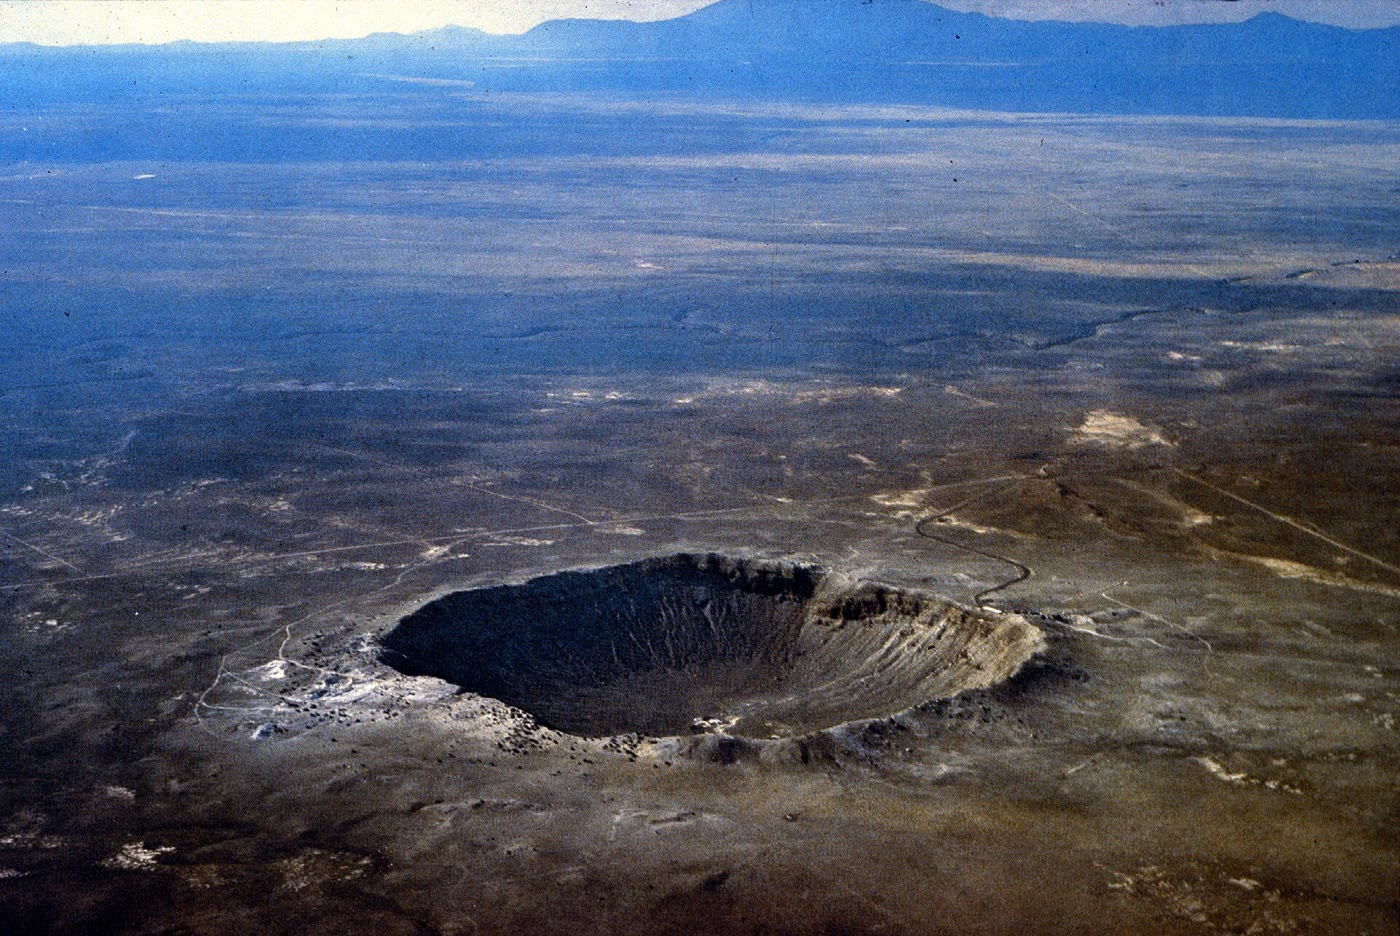
\includegraphics[width=0.66\linewidth]{images/book5/b3-barringer-crater.jpg}
\par\smallskip{\small 亚利桑那州的巴林杰陨石坑，为\omterm{def:b3:planetary-interiors-surfaces:crater-morphology}{简单撞击坑}，
直径 \qty{1.2}{km}，约 50,000 年前由一颗铁陨石形成，
陨石直径约 \qty{30}{m}；坑缘高出高原，\omterm{def:b3:planetary-interiors-surfaces:crater-morphology}{溅射
毯}环绕坑体铺展。航拍照片，USGS/D.~Roddy，公有
领域。}\label{fig:b3:planetary-interiors-surfaces:barringer}
\end{omfigure}
% ledger: photo:b3-barringer, french:barringer

开挖直径 \qty{1}{km} 的撞击坑约需六秒，直径
\qty{200}{km} 的撞击坑约需一分半钟。撞击形成多大的撞击坑，
取决于弹体的能量、重力与岩石的强度；联系它们的规律
由实验与爆炸数据拟合而得，写成无量纲组的乘积形式，
在本阶段不加证明地承认。
其精神在于能量的平衡。
% ledger: french:transient

\begin{proposition}[重力区的标度律]\label{prop:b3:planetary-interiors-surfaces:scaling}
若撞击能量 $E$ 的一固定比例用于将挖掘出的岩石
（密度为 $\rho$）克服重力 $g$ 抬起，则撞击坑的直径按
\[
  D \propto \left(\frac{E}{\rho g}\right)^{1/4} .
\]
\end{proposition}

\begin{proof}
挖出的体积按 $D^3$ 标度，其质量为 $\rho D^3$，并被
抬起的高度量级为 $D$：做功量级为 $\rho g D^4$，
与 $E$ 成正比。
\end{proof}

一部分能量转化为热量、用于熔化和破碎岩石，因此真实规律介于此式与更简单的规则之间：
地球上常被引用的一张表格给出，撞击坑的宽度为
其石质撞击体宽度的二十倍。
重力还决定撞击坑何时不再是\omterm{def:b3:planetary-interiors-surfaces:crater-morphology}{简单撞击坑}。
\omterm{def:b3:planetary-interiors-surfaces:crater-morphology}{瞬态撞击坑}的坑壁在其所承受的岩石重量
（量级为 $\rho g D/3$）超过岩石强度时坍塌，因此
过渡直径与 $1/g$ 成正比：在地球上，结晶岩中约为 \qty{4}{km}，
沉积物中约为 \qty{2}{km}；在月球上约为 \qty{20}{km}，
那里的重力约弱六倍。
% ledger: french:table21, french:transition, planet:Earth.gravity, planet:Moon.gravity

\section{撞击坑定年}\label{sec:b3:planetary-interiors-surfaces:dating}

一个不受扰动的表面，以天体撞击它的速率积累撞击坑。
只要撞击速率已知，数一数撞击坑即可确定表面的年龄，
但所数的撞击坑须确属该表面，而不是
下伏地层或邻近地区抛出的碎屑所形成。

\begin{definition}[撞击坑大小–频率分布]\label{def:b3:planetary-interiors-surfaces:sfd}
表面的\emph{撞击坑大小–频率分布}\index{撞击坑大小–频率分布}是
单位面积上撞击坑数目 $N(D)$（撞击坑直径至少为 $D$），
作为 $D$ 的函数（累积分布），或
按直径分档统计的数目，通常每档直径为上一档的 $\sqrt2$ 倍，
（增量分布）。
\end{definition}

\begin{definition}[撞击坑定年；产生函数与年代函数；平衡密度]\label{def:b3:planetary-interiors-surfaces:crater-dating}
\emph{撞击坑定年}\index{撞击坑定年}是确定表面年龄的方法，
即由撞击坑的密度求得表面的年龄。\emph{撞击坑产生函数}\index{撞击坑产生函数}
是表面所获撞击坑的大小–频率分布的形状，
记为 $F(D) =
N(D)/N(\qty{1}{km})$，并假定其在各个年龄均相同。
\emph{撞击坑年代函数}\index{撞击坑年代函数} $N_1(T)$ 是
单位面积上直径为 \qty{1}{km} 及以上的撞击坑，
在时间 $T$ 内的累积数目。表面处于
某一给定大小撞击坑的\emph{撞击坑平衡密度}\index{撞击坑平衡密度}时，
每一新撞击坑平均抹去的旧撞击坑数恰与其新增数目相等，
其数目不再增长。
\end{definition}

由一次计数即可得出表面的模式年龄：$N(D)$ 为在任一 $D$ 处测得的数目，
由此得 $N_1 = N(D)/F(D)$，而 $T$ 满足 $N_1(T) = N_1$。
$N(D) = N_1(T)F(D)$ 所示的曲线（$T$ 固定）称为等时线。对于火星，
常用的产生函数是以 $\log_{10}D$ 为变量的 11 次多项式，并且
其年代函数的形式为
\[
  N_1(T) = a\left(e^{bT} - 1\right) + cT , \qquad
  a = \qty{3.22e-14}{km^{-2}}, \ b = \qty{6.93}{Ga^{-1}}, \
  c = \qty{4.875e-4}{km^{-2}.Ga^{-1}} ,
\]
在最近三十亿年内近似为线性，更早则呈陡峭的指数增长。
月球的函数具有相同形式，其中 $a = \num{5.44e-14}$ 及 $c =
\num{8.38e-4}$。它依据阿波罗与月球号着陆点的年龄拟合得到；
火星的函数则是将月球的函数，按火星与月球撞击速率之比的估计值
进行换算而得。
% ledger: craterstats:mars-pf, craterstats:mars-cf, craterstats:moon-cf, marchi:neukum

\begin{omfigure}
\centering
\begin{tikzpicture}
\begin{groupplot}[group style={group size=2 by 1, horizontal sep=1.6cm},
  width=0.48\linewidth, height=0.46\linewidth,
  tick label style={font=\scriptsize}, label style={font=\small}, title style={font=\small}]
\nextgroupplot[title={火星的等时线}, xmode=log, ymode=log, xmin=0.1, xmax=100,
  ymin=1e-8, ymax=100, xlabel={撞击坑直径 $D$（\unit{km}）},
  ylabel={$N(D)$，每 \unit{km^2} 中直径 $\geq D$ 的撞击坑数},
  xtick={0.1,1,10,100}, xticklabels={0.1,1,10,100},
  ytick={1e-8,1e-6,1e-4,1e-2,1}]
\addplot[thick, black!50, dashed] table[x=D, y=eq] {figdata/out/bachelor-3-crater_sfd-iso.dat};
\addplot[omDef] table[x=D, y=N_0.1] {figdata/out/bachelor-3-crater_sfd-iso.dat};
\addplot[omDef] table[x=D, y=N_1] {figdata/out/bachelor-3-crater_sfd-iso.dat};
\addplot[omDef] table[x=D, y=N_3.5] {figdata/out/bachelor-3-crater_sfd-iso.dat};
\addplot[red!70!black, thick] table[x=D, y=N_4] {figdata/out/bachelor-3-crater_sfd-iso.dat};
\node[font=\tiny, omDef, anchor=north east] at (axis cs:0.75,8e-6) {0.1~Ga};
\node[font=\tiny, omDef, anchor=north east] at (axis cs:2.6,1e-5) {1~Ga};
\node[font=\tiny, omDef, anchor=north east] at (axis cs:9,3.5e-5) {3.5~Ga};
\node[font=\tiny, red!70!black, anchor=north east] at (axis cs:45,2.5e-5) {4~Ga};
\node[font=\tiny, black!60, anchor=south, rotate=-30] at (axis cs:25,3.5e-4) {平衡};
\nextgroupplot[title={年代函数}, ymode=log, xmin=0, xmax=4.5,
  ymin=1e-5, ymax=0.3, xlabel={年龄 $T$（\unit{Ga}）}, ylabel={每 \unit{km^2} 的 $N_1$},
  legend style={font=\scriptsize, at={(0.03,0.97)}, anchor=north west}]
\addplot[thick, red!70!black] table[x=T, y=mars] {figdata/out/bachelor-3-crater_sfd-chron.dat};
\addlegendentry{火星}
\addplot[thick, black!60, dashed] table[x=T, y=moon] {figdata/out/bachelor-3-crater_sfd-chron.dat};
\addlegendentry{月球}
\end{groupplot}
\end{tikzpicture}
\par\smallskip{\small 左：火星的等时线，即表面年龄为 0.1、1、3.5 和 4 十亿年时的
撞击坑累积密度，另绘平衡密度（虚线），它限制了每一次计数：在 4 十亿年的表面上，
直径小于约 \qty{0.7}{km} 的撞击坑已处于平衡，不再记录年龄。
右：火星与月球的年代函数，即每平方千米中直径
为 \qty{1}{km} 及以上的撞击坑数目，随表面年龄
的变化
关系。
}\label{fig:b3:planetary-interiors-surfaces:sfd}
\end{omfigure}
% ledger: craterstats:mars-pf, craterstats:mars-cf, craterstats:moon-cf, craterstats:equilibrium

撞击随机地、彼此独立地发生，因此在某一面积上所数得的撞击坑数目
$n$ 服从泊松分布。

\begin{proposition}[模式年龄的计数误差]\label{prop:b3:planetary-interiors-surfaces:poisson}
若数得 $n$ 个撞击坑，计数面积为 $A$，则密度 $N = n/A$ 的
标准差为 $\sqrt n/A$，相对误差为 $1/\sqrt n$，模式年龄的
标准差为
\[
  \sigma_T = \frac{N_1(T)}{\sqrt n\,N_1'(T)} .
\]
\end{proposition}

\begin{proof}
泊松变量的均值为 $\lambda$，其方差也为 $\lambda$，由 $n$ 估计。
年龄为 $T = N_1^{-1}(N_1)$；取一阶近似，$\sigma_T =
\sigma_{N_1}/N_1'(T)$，且 $\sigma_{N_1} = N_1/\sqrt n$。
\end{proof}

仅计数本身的相对误差，在一百个撞击坑时为
百分之十。在年轻表面上，$N_1$ 为线性，年龄继承了这一误差：
$\sigma_T/T = 1/\sqrt n$。在古老表面上，陡峭的函数使其缩小为
原来的六分之一，在 \qty{3.8}{Ga} 时（见\cref{exo:b3:planetary-interiors-surfaces:11}）；
古老表面的模式年龄此时转而受限于
函数本身的标定。计数还受两个进一步的限制。小撞击坑会饱和：
在最古老的表面上，直径小于约 \qty{0.7}{km} 的撞击坑
已处于平衡密度，不再记录时间。另外，表面可能被重塑，
而未被抹去：一股熔岩流掩埋了小撞击坑，却未掩埋大撞击坑的
坑缘，形成了一个带有拐点的分布：在大 $D$ 处古老，
在小 $D$ 处年轻。该拐点标示了\omterm{def:b3:planetary-interiors-surfaces:resurfacing}{表面重塑}的时间。
% ledger: craterstats:equilibrium

\begin{definition}[表面重塑]\label{def:b3:planetary-interiors-surfaces:resurfacing}
\emph{表面重塑}\index{表面重塑}是行星表面的重塑，
由熔岩、沉积物、冰或变形造成，它抹去或掩埋其撞击坑，
并重置其撞击坑时钟。
\end{definition}

\section{地球之外的火山作用与构造}\label{sec:b3:planetary-interiors-surfaces:volcanism}

每颗类地行星都通过其岩石圈散失内部热量。
地球借助运动的板块实现这一点，其他行星则采用不同方式。

\begin{definition}[停滞盖]\label{def:b3:planetary-interiors-surfaces:stagnant-lid}
若一颗行星的岩石圈是一个单一的刚性外壳，
不参与其下方地幔的对流：热量经由传导
及穿过它上升的岩浆散失，则称该行星具有\emph{停滞盖}\index{停滞盖}。
在地球这类活动盖行星上，岩石圈被分割为板块，
板块沉回地幔之中。
\end{definition}

\begin{definition}[热管火山作用]\label{def:b3:planetary-interiors-surfaces:heat-pipe}
\emph{热管火山作用}\index{热管火山作用}是一种行星内部热量的散失方式，
主要通过岩浆沿狭窄通道上升，
在地表喷发，熔岩冷却后被后续熔岩掩埋：
岩石圈自顶部增生，并被携带向下，保持低温。
\end{definition}

\begin{omfigure}
\centering
\begin{tikzpicture}[x=0.5cm, y=0.5cm, font=\scriptsize, >=stealth]
\foreach \dx/\name in {0/活动盖, 9.5/停滞盖, 19/热管} {
  \begin{scope}[xshift=\dx*0.5cm]
  \fill[orange!15] (0,0) rectangle (8,4);
  \node[anchor=south] at (4,5.6) {\name};
  \end{scope}}
% mobile lid: plates, ridge, slab
\fill[omDef!35] (0,4) rectangle (3.9,4.8);
\fill[omDef!35] (4.1,4) rectangle (6.2,4.8);
\fill[omDef!35] (6.2,4.8) -- (7.6,1.6) -- (6.9,1.4) -- (5.5,4.0) -- cycle;
\fill[omDef!35] (6.55,4) rectangle (8,4.8);
\draw[->, thick] (3.6,5.1) -- (1.6,5.1); \draw[->, thick] (4.4,5.1) -- (6.0,5.1);
\draw[->, red!70!black] (4,1.0) -- (4,3.6);
\draw[black!60, ->] (2.0,3.4) arc (90:270:1.0 and 1.2);
\node[anchor=north] at (4,-0.2) {板块下沉};
% stagnant lid
\begin{scope}[xshift=4.75cm]
\fill[omDef!35] (0,3.2) rectangle (8,4.8);
\draw[black!60, ->] (2.4,3.0) arc (90:270:1.2 and 1.2);
\draw[black!60, ->] (5.6,0.6) arc (-90:90:1.2 and 1.2);
\fill[red!70!black] (3.9,3.2) rectangle (4.1,4.8);
\fill[red!70!black] (3.0,4.8) -- (4,5.4) -- (5.0,4.8) -- cycle;
\node[anchor=north] at (4,-0.2) {单层厚壳};
\end{scope}
% heat pipe
\begin{scope}[xshift=9.5cm]
\fill[omDef!35] (0,1.0) rectangle (8,4.8);
\foreach \x in {1.5,4,6.5} {\fill[red!70!black] (\x-0.1,1.0) rectangle (\x+0.1,4.8);
  \fill[red!70!black] (\x-0.6,4.8) -- (\x,5.2) -- (\x+0.6,4.8) -- cycle;}
\draw[->, thick] (2.75,4.3) -- (2.75,1.6); \draw[->, thick] (5.25,4.3) -- (5.25,1.6);
\node[anchor=north] at (4,-0.2) {熔岩被掩埋，盖层低温};
\end{scope}
\end{tikzpicture}
\par\smallskip{\small 三种散热方式（示意图）。左：
活动盖，板块在洋中脊形成、在海沟下沉，如
地球。中：\omterm{def:b3:planetary-interiors-surfaces:stagnant-lid}{停滞盖}，单层刚性外壳覆盖在对流地幔之上，
由少数长寿火山的岩浆穿过。右：热管，
岩浆沿狭窄通道穿过厚而冷的岩石圈上升，其熔岩
被后续熔岩掩埋，并被携带
向下。}\label{fig:b3:planetary-interiors-surfaces:lids}
\end{omfigure}

火星具有\omterm{def:b3:planetary-interiors-surfaces:stagnant-lid}{停滞盖}。没有板块把火山从其源区带走，
它的火山长期原地生长于塔尔西斯
隆起之上。奥林帕斯山是太阳系中已知最大的火山，
高 \qty{27}{km}，底座直径超过 \qty{600}{km}，四周环绕着
高达 \qty{6}{km} 的陡坡；附近的三座塔尔西斯火山，各自直径为 350
至 \qty{400}{km}。如此巨大的荷载使岩石圈弯曲，
其所挖凹槽的宽度，与地球上一样，度量了
盖层的弹性厚度。
% ledger: nasa:olympus-mons

\begin{omfigure}
\centering
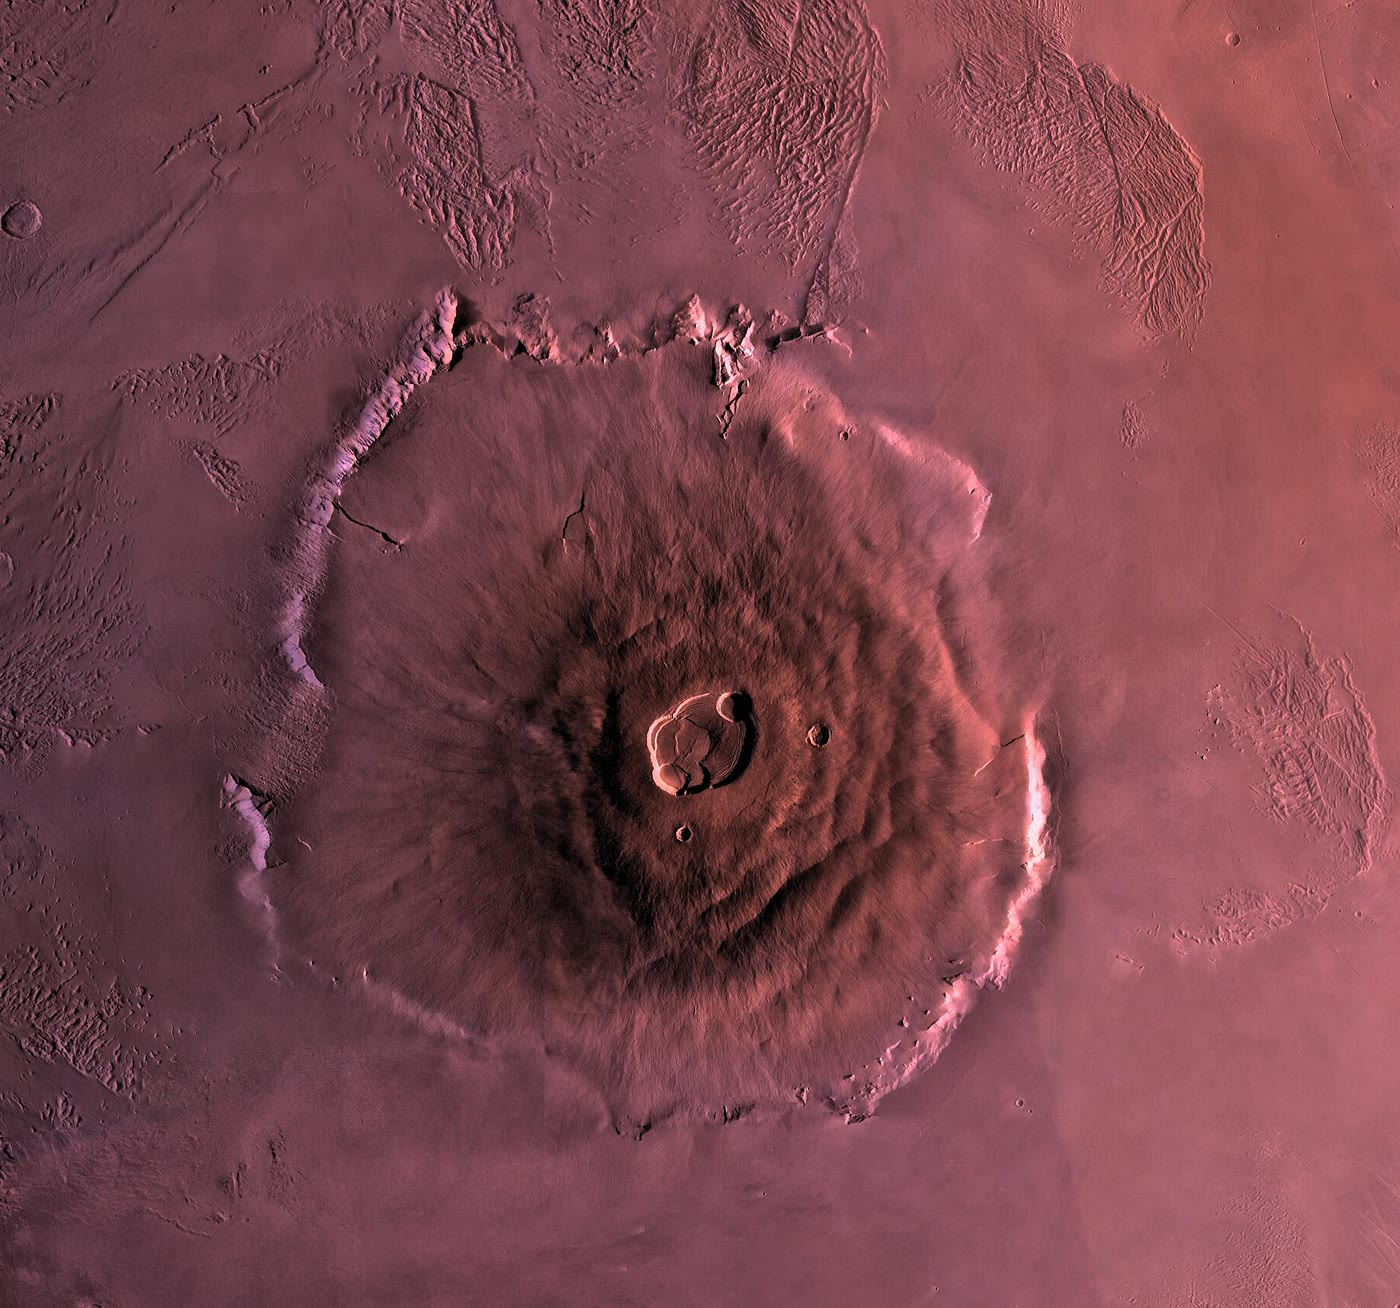
\includegraphics[width=0.48\linewidth]{images/book5/b3-olympus-mons.jpg}
\par\smallskip{\small 火星上的奥林帕斯山，由维京号轨道器图像拼接而成：
顶部破火山口位于中央，熔岩流的侧翼，
以及环绕底部的陡崖状陡坡，直径约 \qty{600}{km}。
NASA/JPL/USGS，公有领域。}\label{fig:b3:planetary-interiors-surfaces:olympus}
\end{omfigure}
% ledger: photo:b3-olympus-mons, nasa:olympus-mons

金星与地球大小相近，其撞击坑数量在
除地球外的所有岩质行星中远为最少。其表面特征的平均年龄可能
仅为 1.5 亿年，其间夹杂着更老的斑块：
火山作用与变形更新了其大部分表面，可能是断续进行的，
历时很长，也可能更快。金星上有数以千计的火山，
却没有板块运动的迹象。
% ledger: nasa:venus-surface, planet:Venus.diameter, planet:Earth.diameter

木卫一是木星最靠内的大卫星，其表面散失的热量超过
\qty{2.5}{W.m^{-2}}，约为地球平均值 \qty{0.092}{W.m^{-2}} 的 27 倍。
其热量并非来自放射性，而是
由潮汐产生。
% ledger: veeder:io-heat, dd10:split

\begin{definition}[潮汐加热]\label{def:b3:planetary-interiors-surfaces:tidal-heating}
\emph{潮汐加热}\index{潮汐加热}是指天体内部由变化的潮汐施加的形变
所引起的摩擦而产生的热量。
处于同步自转、轨道偏心的卫星，
其行星的潮汐强度在每一轨道周期内发生变化，并来回摆动。
\end{definition}

\begin{proposition}[同步卫星的潮汐功率]\label{prop:b3:planetary-interiors-surfaces:tidal-power}
半径为 $R$、处于同步自转的卫星，在平均角速度为
$n$、偏心率为小量 $e$ 的轨道上，耗散的功率为
\[
  \dot E = \frac{21}{2}\,\frac{k_2}{Q}\,\frac{(nR)^5}{G}\,e^2 ,
\]
其中 $Q$ 为该卫星的潮汐品质因数，使得 $k_2/Q$ 度量
以热量形式损失的那部\omterm{def:b3:ocean-dynamics:tides}{分潮}汐形变。
\end{proposition}

该命题在本阶段不加证明地承认。耗散能量的潮汐也会使轨道变圆；
木卫一的轨道仍为椭圆，偏心率为 0.004，这是因为木卫二与木卫三的
拉力时刻精确，对其轨道产生摄动，它们的轨道周期分别为
1.77、3.55 和 \num{7.15}~天，几乎恰好呈 1:2:4 的关系（见\cref{exo:b3:planetary-interiors-surfaces:8}）。
木卫一的表面每个轨道周期内起伏可达
\qty{100}{m}。火山喷发以快于撞击坑形成的速度覆盖其表面；
关于其热量如何散失，一种模型是\omterm{def:b3:planetary-interiors-surfaces:heat-pipe}{热管火山作用}，
它会使一层厚而冷的岩石圈
位于其炽热表面之下。
% ledger: nasa:galilean-orbits, beuthe:tidal-power, nasa:io-orbit, nasa:io-facts

\begin{definition}[地下海洋]\label{def:b3:planetary-interiors-surfaces:ocean-world}
\emph{地下海洋}\index{地下海洋}是一层全球性的
位于卫星或矮行星冰壳之下的液态水层，
由\omterm{def:b3:planetary-interiors-surfaces:tidal-heating}{潮汐加热}和放射性加热维持其液态。
\end{definition}

\begin{definition}[冰火山作用]\label{def:b3:planetary-interiors-surfaces:cryovolcanism}
\emph{冰火山作用}\index{冰火山作用}是指水、卤水
或其他挥发性液体与蒸气（而非熔岩）的喷发，
出现在卫星或矮行星的冰质表面上。
\end{definition}

木卫二的冰壳经朱诺号探测器的微波辐射计在其飞越区域测得，
平均厚约 \qty{29}{km}；其下是一片咸水海洋，
所含水量为地球全部海洋的两倍。土星的卫星土卫二
直径仅约 \qty{500}{km}，2005 年卡西尼号探测器
在其南极附近发现，冰粒与气体的喷流
从温暖的裂缝中喷出，速度约为 \qty{400}{m.s^{-1}}。
其引力与自转的摆动表明，
这些喷流源自一片全球性海洋，
海洋上覆冰壳平均厚 20 至 \qty{25}{km}，
而在南极处可能仅厚 1 至 \qty{5}{km}。
% ledger: jpl:europa-shell, nasa:europa-ocean, nasa:enceladus

\section{大核与小核}\label{sec:b3:planetary-interiors-surfaces:cores}

四个已测得的地核构成一个奇特的家族。
以其半径为基准，地球的地核到达表面距离的 0.55，火星为 0.54；
月球为 0.19；水星为 0.82。行星分异（见本科二年级分册）可以将
每个天体内部的金属与硅酸盐分开，但无法使金属的比例差异如此之大。
巨大撞击却可以做到。据信月球是约 45 亿年前，
由一颗与火星大小相当的天体与年轻的地球相撞后形成的碎片聚集而成，
撞击体的金属并入地球的地核，而月球主要聚集了地幔岩石，
因此其地核很小。类似的撞击可能剥离了水星大部分的硅酸盐地幔，
使其成为富铁的行星，其地核几乎占据整个天体。
地核与撞击坑一样，
记录着一段碰撞的历史。
% ledger: data:prem, jpl:insight-interior, nasa:moon-core, agu:mercury-core, french:giant-impacts

\section{练习}

\begin{exercise}[$\star$]\label{exo:b3:planetary-interiors-surfaces:1}
水星的平均密度为 \qty{5429}{kg.m^{-3}}，转动惯量因子为 0.35，
半径为 \qty{2440}{km}。取两层模型，地幔密度为
\qty{3300}{kg.m^{-3}}，求地核的相对半径、其半径（以千米计）
及其密度。
\end{exercise}

\begin{exercise}[$\star$]\label{exo:b3:planetary-interiors-surfaces:2}
一颗直径为 \qty{50}{m}、密度为 \qty{3500}{kg.m^{-3}} 的石质弹体，
以 \qty{20}{km.s^{-1}} 的速度竖直撞击地球。求其质量及其动能，
分别以焦耳和百万吨炸药当量表示，
（$\qty{1}{Mt} = \qty{4.2e15}{J}$）。按照二十倍弹体直径的规则，
所得撞击坑的直径是多少？
\end{exercise}

\begin{exercise}[$\star$]\label{exo:b3:planetary-interiors-surfaces:3}
在面积为 \qty{100000}{km^2} 的火星平原上，
计得直径为 \qty{1}{km} 及以上的撞击坑 120 个。求 $N_1$、其相对误差，
以及该平原的模式年龄及其误差。
\end{exercise}

\begin{exercise}[$\star$]\label{exo:b3:planetary-interiors-surfaces:4}
木卫一半径为 \qty{1821.5}{km}，散热速率为 \qty{2.5}{W.m^{-2}}。求其
总散热量，并将其与地球的 \qty{47}{TW} 进行比较，
分别比较总量以及每平方米的散热量（地球为 \qty{0.092}{W.m^{-2}}）。
\end{exercise}

\begin{exercise}[$\star\star$]\label{exo:b3:planetary-interiors-surfaces:5}
火星质量为 \qty{6.417e23}{kg}，半径为 \qty{3389.5}{km}。
(a)~求其平均密度、表面重力加速度以及 $\rho gR$。
(b)~将其视为刚度为 \qty{67}{GPa} 的均匀不可压缩球体，
求其\omterm{def:b3:planetary-interiors-surfaces:love-number}{勒夫数} $k_2$。
(c)~实测值为 $0.153 \pm 0.017$。该比较说明了什么？
\end{exercise}

\begin{exercise}[$\star\star$]\label{exo:b3:planetary-interiors-surfaces:6}
在地球上（$g = \qty{9.8}{m.s^{-2}}$），\omterm{def:b3:planetary-interiors-surfaces:crater-morphology}{简单撞击坑}向\omterm{def:b3:planetary-interiors-surfaces:crater-morphology}{复杂撞击坑}的过渡
约在晶质岩石中为 \qty{4}{km}，在
沉积物中为 \qty{2}{km}。(a)~假设过渡直径与 $1/g$ 成正比，
据此预测其在月球（$g = \qty{1.62}{m.s^{-2}}$）以及火星和
水星（$g = \qty{3.7}{m.s^{-2}}$）上的数值，并与月球上观测到的 \qty{20}{km}
相比较。(b)~若塌陷在 $\rho gD/3$ 超过
岩石强度 $Y$ 时开始，则地球晶质岩石过渡所给出的强度为多少
（取 $\rho = \qty{2600}{kg.m^{-3}}$）？
\end{exercise}

\begin{exercise}[$\star\star$]\label{exo:b3:planetary-interiors-surfaces:7}
某表面上直径为 \qty{1}{km} 及以上的撞击坑数为每平方千米 $\num{2.0e-3}$
个。用火星的\omterm{def:b3:planetary-interiors-surfaces:crater-dating}{撞击坑年代函数}求其模式年龄，
通过数值求解方程。若改用月球的\omterm{def:b3:planetary-interiors-surfaces:crater-dating}{撞击坑年代函数}，
所得年龄为多少，两者为何不能互换？
\end{exercise}

\begin{exercise}[$\star\star$]\label{exo:b3:planetary-interiors-surfaces:8}
木卫一、木卫二与木卫三的轨道周期分别为 1.769138、3.551181 和
\num{7.154553}~天。(a)~计算相邻周期之比。
(b)~计算 $1/P_I - 3/P_E + 2/P_G$，并加以评论。(c)~为何共振能
维持潮汐原本会消除的偏心率？
\end{exercise}

\begin{exercise}[$\star\star$]\label{exo:b3:planetary-interiors-surfaces:9}
木卫一绕木星运行的周期为 \num{1.769138}~天，偏心率为 0.004。
求潮汐功率命题给出的、每单位 $k_2/Q$ 的功率，
以及能提供木卫一
的散热量（见\cref{exo:b3:planetary-interiors-surfaces:4}）所需的 $k_2/Q$ 值。
\end{exercise}

\begin{exercise}[$\star\star\star$]\label{exo:b3:planetary-interiors-surfaces:10}
对月球，$\bar\rho = \qty{3340}{kg.m^{-3}}$，$C = 0.394$。
(a)~在两层模型中证明 $\mathrm dx^2/\mathrm dC =
\tfrac52\bar\rho/(\bar\rho - \rho_m)$（$\rho_m$ 固定）。(b)~
取使地核 $x = 0.19$ 的地幔密度 \qty{3288}{kg.m^{-3}}，
求 $x$ 与 $\rho_c$ 分别在 $C = 0.395$ 和 $C = 0.393$ 时的值？
(c)~这对用转动惯量称量小地核
说明了什么？
\end{exercise}

\begin{exercise}[$\star\star\star$]\label{exo:b3:planetary-interiors-surfaces:11}
(a)~对 100 个撞击坑，计算一个年龄为
\qty{1.0}{Ga} 的火星表面与一个年龄为 \qty{3.8}{Ga} 的火星表面的模式年龄计数误差。
(b)~证明在\omterm{def:b3:planetary-interiors-surfaces:crater-dating}{撞击坑年代函数}的线性段上，$\sigma_T/T =
1/\sqrt n$。(c)~那么古老表面的年龄为何仍不确定？
\end{exercise}

\begin{exercise}[$\star\star\star$]\label{exo:b3:planetary-interiors-surfaces:12}
木卫二半径为 \qty{1560.8}{km}，绕木星运行周期为 \num{3.551181}~天，
偏心率为 0.009。(a)~若木卫二耗散潮汐所用的 $k_2/Q$ 与木卫一相同，
则其产生的潮汐功率为木卫一的多大比例，热流又为多少？
(b)~对于冰下存在海洋的卫星，该假设为何存疑？
\end{exercise}

\section{问题：火星上的两片平原}

\begin{problem}[{周末问题——火星的地核与两片
虚构熔岩平原的年龄}]
\label{pb:b3:planetary-interiors-surfaces:1}
火星质量为 \qty{6.4169e23}{kg}，半径为 \qty{3389.5}{km}，以及
转动惯量因子为 0.366。两片虚构平原 A 与 B 位于其
火山区上，其撞击坑已在图像上按
上下限之比为 $\sqrt2$ 的直径区间统计。

\medskip\noindent\textbf{第一部分——地核。}
\begin{enumerate}
\item 计算火星的平均密度。
\item 采用两层模型，地幔密度取 \qty{3500}{kg.m^{-3}}，计算
  地核的相对半径、以千米计的半径及其
  密度。
\item InSight 测得地核半径为 \qty{1830}{km}，则
  两层模型所需的地幔与地核密度各为多少？
\item 将该地核密度与地球外核
  顶部之下的密度 \qty{9900}{kg.m^{-3}}（取自地球参考模型）相比较，
  并说明为何火星上预期数值更低，以及它还
  暗示了什么。
\item 火星在刚度为
  \qty{67}{GPa} 时的均匀球体\omterm{def:b3:planetary-interiors-surfaces:love-number}{勒夫数}为 0.109，实测值为 0.153。哪一项观测先得出，
  它已对地核说明了什么？
\item 火星地壳厚 20 至 \qty{37}{km}。它占
  整个行星体积的多大比例？忽略它是否合理？
\end{enumerate}

\medskip\noindent\textbf{第二部分——平原 A 上的计数。}平原 A
面积为 \qty{80000}{km^2}。其撞击坑按直径区间（千米）统计如下：
\begin{center}
\small
\begin{tabular}{lccccccccc}
\hline
直径区间 & 1--1.41 & 1.41--2 & 2--2.83 & 2.83--4 & 4--5.66 & 5.66--8 & 8--11.3 & 11.3--16 & 16--22.6 \\
\hline
平原 A & 38 & 6 & 5 & 3 & 0 & 0 & 0 & 1 & 1 \\
平原 B & 48 & 8 & 31 & 12 & 7 & 2 & 0 & 2 & 2 \\
\hline
\end{tabular}
\end{center}
\begin{enumerate}[resume]
\item 计算平原 A 自 \qty{1}{km} 起的累积计数。
\item 计算每平方千米的 $N(\qty{1}{km})$ 及其
  标准差。
\item \omterm{def:b3:planetary-interiors-surfaces:crater-dating}{撞击坑产生函数}给出 $F(\qty{2}{km}) = 0.147$ 与
  $F(\qty{1.41}{km}) = 0.355$。在 1.41 与 \qty{2}{km} 处的计数
  是否与产生函数的形状相符？
\item 平原 A 是否接近\omterm{def:b3:planetary-interiors-surfaces:crater-dating}{撞击坑平衡密度}，
  即 \qty{1}{km} 处的 \qty{0.072}{km^{-2}}？
\item 为何选取上下限之比为 $\sqrt2$ 的分档？
\item 成群与成链的小撞击坑不计入统计。为什么？
\end{enumerate}

\medskip\noindent\textbf{第三部分——模式年龄。}使用火星的\omterm{def:b3:planetary-interiors-surfaces:crater-dating}{撞击坑
年代函数}。
\begin{enumerate}[resume]
\item 计算平原 A 的模式年龄。检验指数项
  可以忽略。
\item 计算其计数误差。
\item 若采用月球的年代学，会得到什么年龄？
\item 平原 B 的面积为 \qty{120000}{km^2}。利用其中直径为
  \qty{2}{km} 及以上的撞击坑，计算 $N(\qty{2}{km})$，再求 $N_1$，
  然后通过数值求解方程，得到其模式年龄。
\item 计算该年龄的计数误差。
\item 比较两个年龄的相对误差，并解释其
  差异。
\end{enumerate}

\medskip\noindent\textbf{第四部分——平原 B 中被掩埋的撞击坑。}
\begin{enumerate}[resume]
\item 若平原 B 的整个表面具有第 16 题的年龄，则其中 1 至 \qty{2}{km} 之间的撞击坑
  应有多少个？实际有多少个？
\item 假设熔岩在时刻 $T_r$ 掩埋了所有直径小于 \qty{2}{km} 的撞击坑，
  而保留了较大的撞击坑，利用
  \num{1}--\qty{2}{km} 的撞击坑计算 $T_r$。
\item 计算 $T_r$ 的计数误差。
\item 设火星上一个新鲜\omterm{def:b3:planetary-interiors-surfaces:crater-morphology}{简单撞击坑}的深度为其宽度的
  五分之一（本题的假设）。熔岩须有多厚才能掩埋
  一个 \qty{2}{km} 的撞击坑，较大的撞击坑为何仍然可见？
\item 平原 B 的熔岩与平原 A 的熔岩能否属于同一期
  火山活动？
\item 以十亿年为单位，给出平原 A 的模式年龄，
  保留两位有效数字。
\end{enumerate}
\end{problem}
% ledger: nasa:mars, jpl:insight-interior, yoder:mars-k2, data:prem, craterstats:mars-pf, craterstats:mars-cf, craterstats:moon-cf, craterstats:equilibrium
